\documentclass{article}
\usepackage{graphicx}
\usepackage{color}
\usepackage{tikz}
\usepackage{amsmath}
\usepackage{listings}
\usepackage{hyperref}
\usepackage{subcaption}

\title{Project}
\author{Masoumeh Ghadamgahi}
\date{\today}

\lstset{ %
  language=R,                   % Specify the language
  basicstyle=\footnotesize,      % The size of the fonts that are used for the code
  numbers=left,                 % Where to put the line numbers
  numberstyle=\tiny\color{gray}, % Style of the line numbers
  stepnumber=1,                 % Number every line
  numbersep=5pt,                % How far the line numbers are from the code
  backgroundcolor=\color{white}, % Choose the background color
  showspaces=false,             % Show spaces adding particular underscores
  showstringspaces=false,       % Underline spaces within strings
  showtabs=false,               % Show tabs within strings adding particular underscores
  frame=single,                 % Adds a frame around the code
  tabsize=2,                    % Default tab size
  captionpos=b,                 % Position of the caption
  breaklines=true,              % Automatic line breaking
  breakatwhitespace=false,      % Automatic breaks should only happen at spaces
  escapeinside={\%*}{*)}        % Escape to LaTeX using the symbols \%* and *)
}

\begin{document}

\maketitle

\section*{Image Processing, Wordclouds and Network Graphs}

In this section, we show the R code and its corresponding output for image processing, word clouds, and network graphs.

\subsection*{Image Processing}

The following is the R code for image processing using the magick library. It scales and annotates an image.

\begin{lstlisting}[language=R]
library(magick)
image <- image_read("C:/Users/user/Pictures/masoumeh.jpg")
print(image)
image_scale(image, "600")
image_scale(image, "x600")
image <- image_scale(image, "x600")
image <- image_modulate(image, brightness = 100, saturation = 90, hue = 100)
image_annotate(image, "Masoumeh", size = 30, color = "brown", boxcolor = "ivory", font = "Forte", strokecolor = "black", degrees = 0, location = "+300+0")
\end{lstlisting}

Here is the output image after processing:

\begin{figure}[h!]
  \centering
  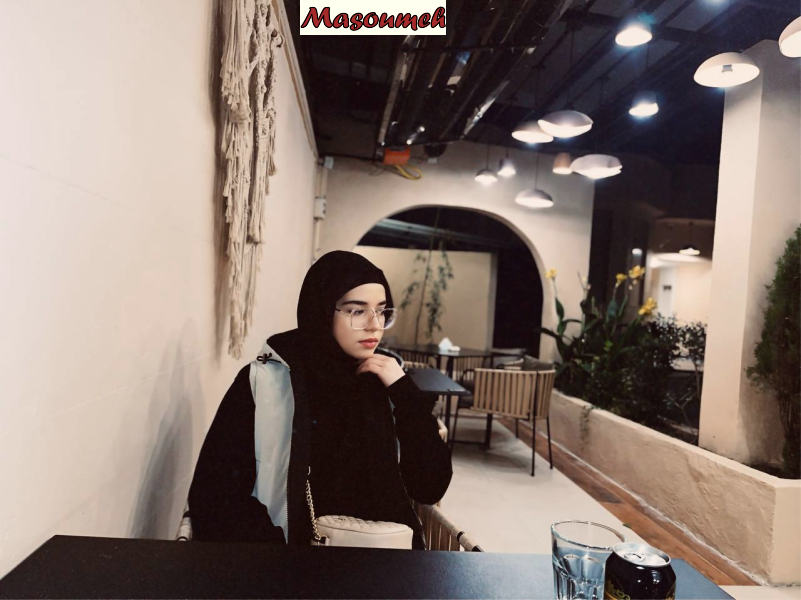
\includegraphics[width=0.8\textwidth]{masoumeh.jpg} % Replace with the name of your image
  \caption{Processed Image: Masoumeh}
  \label{fig:processed_image}
\end{figure}

\newpage

\subsection*{Wordcloud Examples}

Below is the R code used to generate word clouds from text data.

\begin{lstlisting}[language=R]
library("tm")
library("SnowballC")
library("wordcloud")
library("RColorBrewer")
library("wordcloud2")

text <- readLines(file.choose())
docs <- Corpus(VectorSource(text))
docs <- tm_map(docs, content_transformer(tolower))
docs <- tm_map(docs, removePunctuation)
toSpace <- content_transformer(function(x, pattern) gsub(pattern, " ", x))
docs <- tm_map(docs, toSpace, "/")
docs <- tm_map(docs, removeNumbers)
docs <- tm_map(docs, removeWords, c("and", "the", "these", "over", "have", "also", "one", "are", "for", "that", "can", "all", "with", "has", "froms", "from"))

dtm <- TermDocumentMatrix(docs)
m <- as.matrix(dtm)
v <- sort(rowSums(m), decreasing = TRUE)
d <- data.frame(word = names(v), freq = v)

set.seed(200)
wordcloud(words = d$word, freq = d$freq, min.freq = 1, max.words = 150, random.order = FALSE, rot.per = 0.5, colors = brewer.pal(8, "Dark2"))
wordcloud2(data = d, size = 0.7, shape = "star", color = "white", backgroundColor = "blue", minRotation = -pi/6, maxRotation = -pi/6, rotateRatio = 0)
wordcloud2(data = d, size = 0.7, shape = "cardioid", color = "red", backgroundColor = "white", minRotation = -pi/6, maxRotation = -pi/6, rotateRatio = 1)
\end{lstlisting}

The following are the wordcloud outputs generated from the code above:

\begin{figure}[h!]
  \centering
  \begin{minipage}{0.45\textwidth}
    \centering
    
\includegraphics[width=\textwidth]{wordcloud_star.png} % Replace with the name of your first wordcloud image
    \caption{Star-Shaped Wordcloud}
    \label{fig:wordcloud_star}
  \end{minipage} \hfill

𝐌𝐚𝐬𝐨𝐮𝐦𝐞𝐡 𝐒𝐚𝐝𝐚𝐭, [14/10/1403 11:14 ق.ظ]
\begin{minipage}{0.45\textwidth}
    \centering
    
\includegraphics[width=\textwidth]{wordcloud_cardioid.png} % Replace with the name of your second wordcloud image
    \caption{Cardioid-Shaped Wordcloud}
    \label{fig:wordcloud_cardioid}
  \end{minipage}
\end{figure}

\newpage

\subsection*{Network Graph Examples}

The following R code is used to create network graphs from the data:

\begin{lstlisting}[language=R]
library(igraph)
library("readxl")
data <- read_excel("C:/Users/user/Documents/data.xlsx")
x <- data.frame(data$Name, data$City)
net <- graph.data.frame(x, directed = TRUE)
V(net)
E(net)
V(net)$label <- V(net)$name
V(net)$degree <- degree(net)

hist(V(net)$degree, col = 'blue', main = 'Histogram of Node Degree', ylab = 'Frequency', xlab = 'Degree of Vertices')

set.seed(100)
plot(net, vertex.color = 'red', vertex.size = 2, edge.arrow.size = 0.5, vertex.label.cex = 0.8)
plot(net, vertex.color = rainbow(52), vertex.size = V(net)$degree * 3, edge.arrow.size = 1, layout = layout.fruchterman.reingold)
\end{lstlisting}

The following are the network graph outputs generated from the code above:

\begin{figure}[h!]
  \centering
  \begin{minipage}{0.45\textwidth}
    \centering
    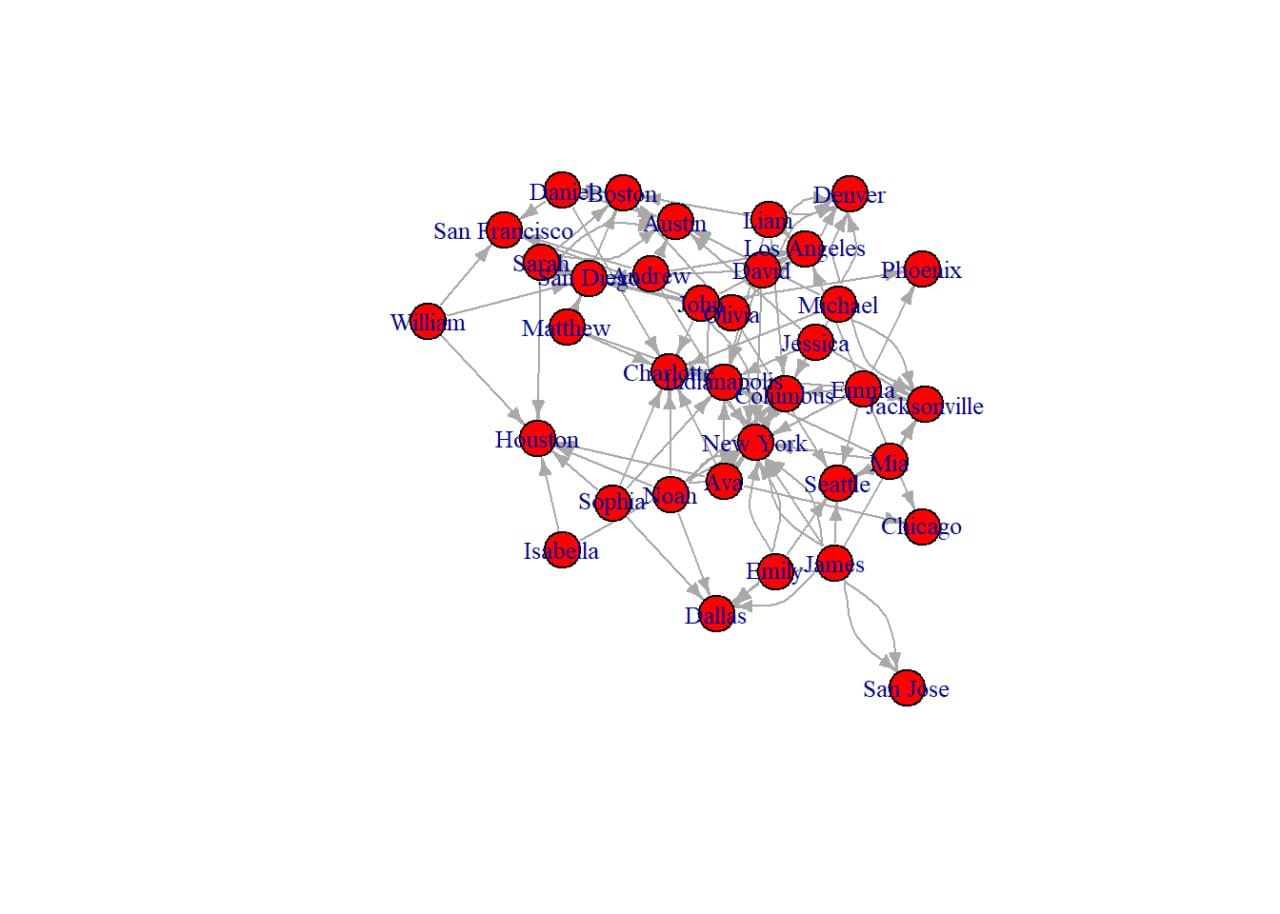
\includegraphics[width=\textwidth]{network_graph_1.png} % Replace with the name of your first network graph image
    \caption{Network Graph Example 1}
    \label{fig:networkgraph_1}
  \end{minipage} \hfill
  \begin{minipage}{0.45\textwidth}
    \centering
    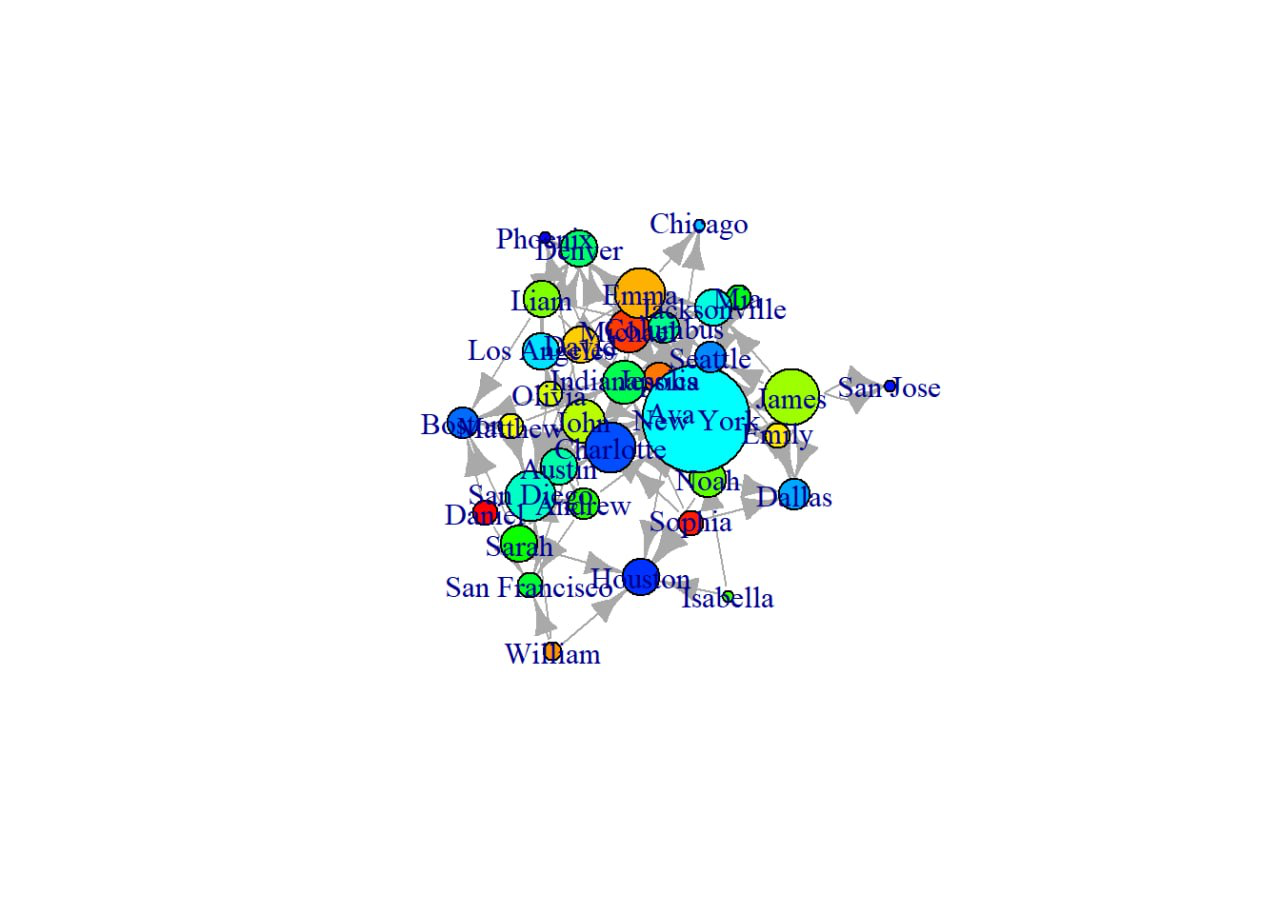
\includegraphics[width=\textwidth]{network_graph_2.png} % Replace with the name of your second network graph image
    \caption{Network Graph Example 2}
    \label{fig:networkgraph_2}
  \end{minipage}
\end{figure}

\end{document}